\section{Session 6: Introduction to linear programming}


%%%%%%%%%%%%%%%%%%%%%%%%%%%%%%%%%%%%%%%%%%%%%%%%%%%%%%%%%%%%%%%%%%%%%%%%%%%%%
%%%%%%%%%%%%%%%%%%%%%%%%%%%%%%%%%%%%%%%%%%%%%%%%%%%%%%%%%%%%%%%%%%%%%%%%%%%%%
%%%%%%%%%%%%%%%%%%%%%%%%%%%%%%%%%%%%%%%%%%%%%%%%%%%%%%%%%%%%%%%%%%%%%%%%%%%%%

\begin{itemize}
  \item Learn how to formulate a linear programming model
  \item Get familiar with the terms feasible region, feasiblke solutions and optimal feasible solutions
  \item Managing graphical solution of the linear programming model
  \item Identify models with unique, multiple or no optimal feasible solutions
  \item Introducing the Simplex method
\end{itemize}


    Linear programs have a linear objective function and linear constraints, which may
    include both equalities and inequalities. The feasible set is a polytope, that is, a convex,
    connected set with flat, polygonal faces. The contours of the objective function are planar.
   \cite{nocedal_numerical_2006}

  A wide variety of applications can be modeled with linear programming.


  Steps:
\begin{enumerate}
  \item identify the controllable decision variables $x_i$, with $i=1,\ldots,n$.
  \item establish the objective criterion: to either maximize or minimize some function of the form:
  \[
    z = c_1 x_1 +\cdots + c_n x_n = \sum_{i=1}^n c_i x_i
  \]
  where $c_i$ represents problem dependent constants.
  \item resource limitations and bounds on decision variables as linear equations or inequalities like
  \[
     a_1 x_1 +\cdots + a_n x_n \leq b
  \]
\end{enumerate}

  \begin{center}
    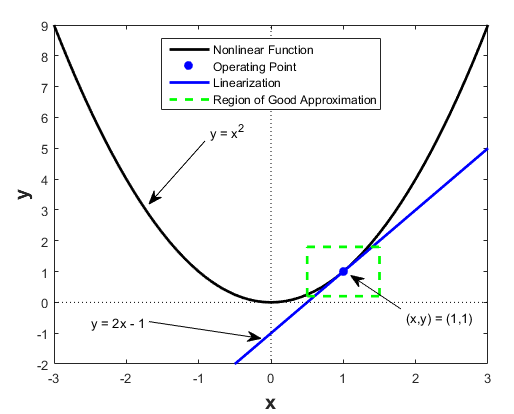
\includegraphics[width=0.45\linewidth]{linearization}
    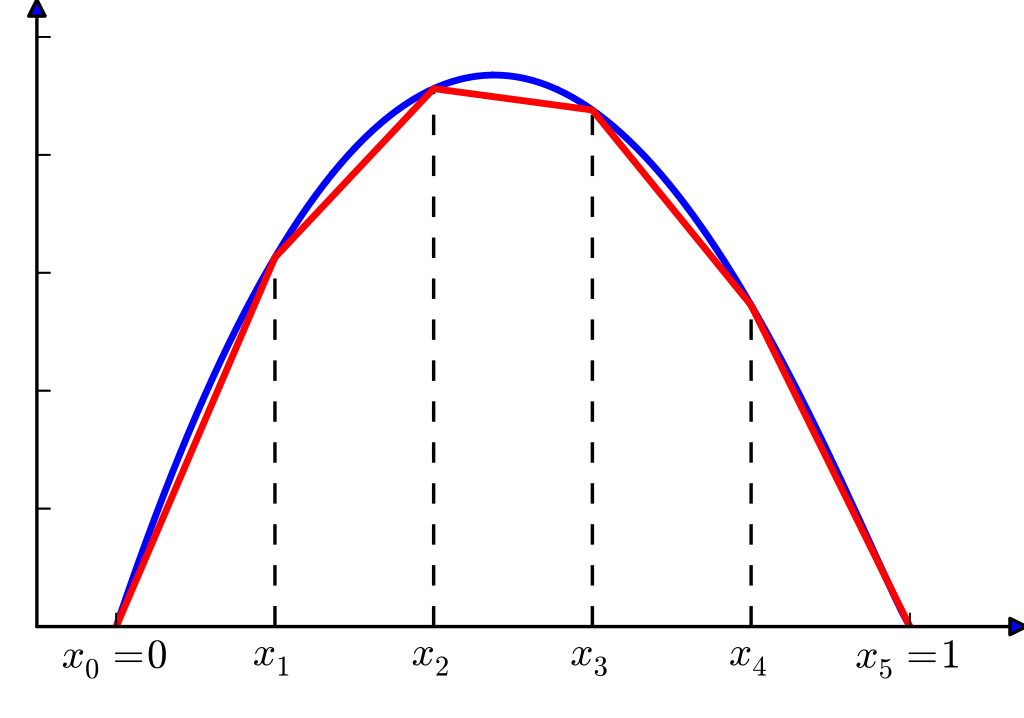
\includegraphics[width=0.45\linewidth]{PWLapprox}

  \href{https://es.mathworks.com/help/slcontrol/ug/linearizing-nonlinear-models.html}{Matlab example}
  \end{center}

  \begin{Exercise}
    A manufacturer of computer system components assembles two models of wireless routers, model A and model B. The amounts of materials and labor required for each assembly, and the total amounts available, are shown in the following table. The profits that can be realized from the sale of each router are \$22 and \$28 for models A and B, respectively, and we assume there is a market for as many routers as can be manufactured.\cite{carter_operations_2019}
    \begin{center}
    \begin{tabular}{cccc}
      & Resources  & Resources  B & Resources  \\
      & per Unit A &  per Unit B &  available \\\hline
      Materials & 8 & 10 & 3400\\
      Labor & 2 & 3 & 960\\\hline
    \end{tabular}
  \end{center}
  How to maximize the benefits?
  \end{Exercise}
  \begin{equation*}
    \begin{aligned}
      \text{maximize } \quad & z = 22 x_A+28x_B \\
      \text{subject to }\quad &
      \begin{array}{rcl}
        8x_A+10x_B &\leq &3400 \\
        2x_A+3x_B &\leq &960 \\
        x_A &\geq &0 \\
        x_B &\geq& 0
      \end{array}
    \end{aligned}
  \end{equation*}


  \begin{Exercise}
  A company wishes to minimize its combined costs of production and inventory over a four-week time period. An item produced in a given week is available for consumption during that week, or it may be kept in inventory for use in later weeks. Initial inventory at the beginning of week 1 is 250 units. The minimum allowed inventory carried from one week to the next is 50 units. Unit production cost is \$15, and the cost of storing a unit from one week to the next is \$3. The following table shows production capacities and the demands that must be met during each week.\cite{carter_operations_2019}
    \begin{center}
    \begin{tabular}{ccc}
      Period  & Production capacity & Demand  \\\hline
      1 &  800 &  900 \\
      2 & 700 & 600\\
      3 & 600 & 800\\
      4 & 800 & 600
    \end{tabular}
  \end{center}
  A minimum production of 500 items per week must be maintained. Inventory costs are not applied to items remaining at the end of the fourth production period, nor is the minimum inventory restriction applied after this final period.
  \end{Exercise}
  Let $x_i$ be the number of units produced during the $i^{th}$ week, for $i = 1, …, 4$. The formulation is somewhat more manageable if we let $A_i$ denote the number of items remaining at the end of each week (accounting for those held over from previous weeks, those produced during the current week, and those consumed during the current week). Note that the $A_i$ values are not decision variables, but merely serve to simplify our written formulation. Thus,
  \begin{eqnarray*}
    A_1&=&250+x_1-900\\
    A_2&=&A_1+x_2-600\\
    A_3&=&A_2+x_3-800\\
    A_4&=&A_3+x_4-600
  \end{eqnarray*}
  \begin{equation*}
    \begin{aligned}
      \text{minimize } \quad & z = 15\cdot(x_1+x_2+x_3+x_4)+3\cdot (A_1+A_2+A_3) \\
      \text{subject to }\quad &
      \begin{array}{c}
        500 \leq x_1 \leq 700\\
        500 \leq x_2 \leq 700\\
        500 \leq x_3 \leq 600\\
        500 \leq x_4 \leq 800\\
        x_i \geq 0, \, i=1,2,3,4
      \end{array}
    \end{aligned}
  \end{equation*}


  \begin{center}
    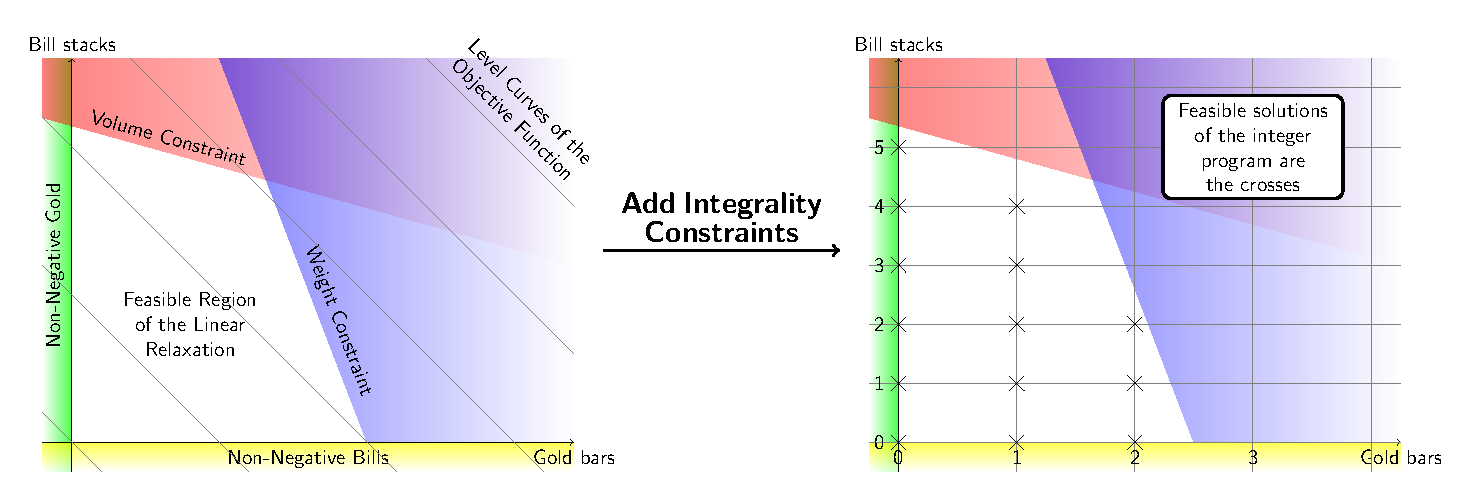
\includegraphics[width=\linewidth]{ILP.pdf}

    \href{http://www.science4all.org/article/integer-programming/}{from Lê Nguyên Hoang's http://www.science4all.org}
  \end{center}

\subsection{Graphical solution}

  \begin{itemize}
    \item Remember: An optimal feasible solution is a point in the feasible space that is as effective as any other point in achieving the specified goal.
    \item The solution of linear programming problems with only two decision variables can be illustrated graphically.
    \item If an optimal feasible solution exists, it occurs at one of the extreme points of the feasible space.
    \item We illustrate this for problems with one, with multiple, and with none optimal feasible solutions.
  \end{itemize}

  \begin{Exercise}
    \begin{equation*}
      \begin{aligned}
        \text{maximize } \quad & z = 3x_1 + x_2 \\
        \text{subject to }\quad &
        \begin{array}{rcl}
          x_2 & \leq & 5\\
          x_1 + x_2 &\leq& 10\\
          -x_1+x_2 &\geq& -2\\
          x_1,x_2 &\geq &0
        \end{array}
      \end{aligned}
    \end{equation*}
  \end{Exercise}
  \begin{center}
    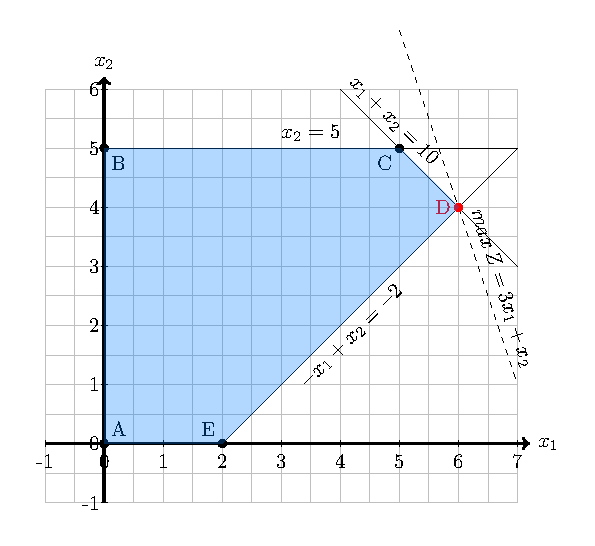
\includegraphics[width=0.6\linewidth]{LP2.pdf}
  \end{center}
  \begin{Exercise}
    \begin{equation*}
      \begin{aligned}
        \text{minimize } \quad & z = x_1 + x_2 \\
        \text{subject to }\quad &
        \begin{array}{rcl}
          3x_1 + x_2 & \geq & 6\\
          x_2 &\geq& 3\\
          x_1 &\leq& 4\\
          x_1,x_2 &\geq &0
        \end{array}
      \end{aligned}
    \end{equation*}
  \end{Exercise}

  \begin{center}
    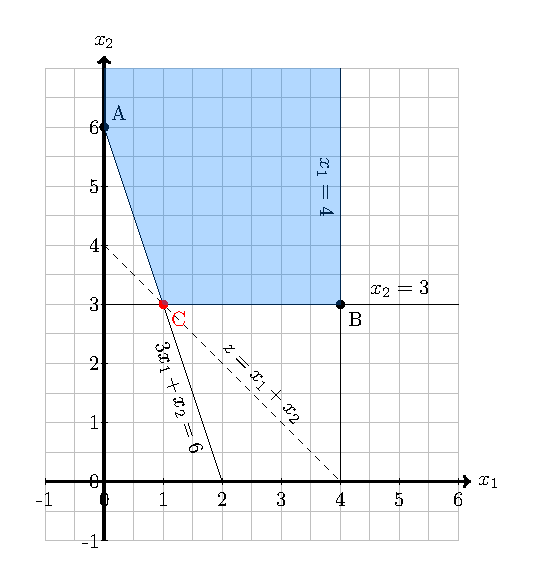
\includegraphics[width=0.6\linewidth]{LP6.pdf}
  \end{center}


  \begin{Exercise}
    \begin{equation*}
      \begin{aligned}
        \text{maximize } \quad & z = x_1 + 2x_2 \\
        \text{subject to }\quad &
        \begin{array}{rcl}
          -x_1+x_2 & \leq & 2\\
          x_1 + 2x_2 &\leq& 8\\
          x_1 &\leq& 6\\
          x_1,x_2 &\geq &0
        \end{array}
      \end{aligned}
    \end{equation*}
  \end{Exercise}
  %
  \begin{center}
   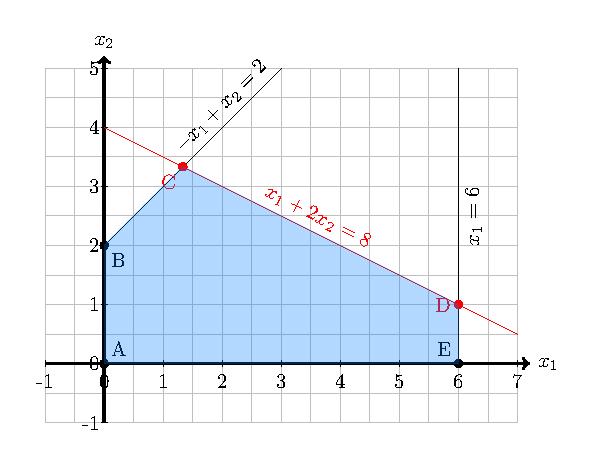
\includegraphics[width=0.7\linewidth]{LP3.pdf}
  \end{center}


  \begin{Exercise}
    \begin{equation*}
      \begin{aligned}
        \text{maximize } \quad & z = 3x_1 + x_2 \\
        \text{subject to }\quad &
        \begin{array}{rcl}
          x_1+x_2 & \geq & 4\\
          -x_1 + x_2 &\leq& 4\\
          -x_1 +2x_2 &\geq& -4\\
          x_1,x_2 &\geq &0
        \end{array}
      \end{aligned}
    \end{equation*}
  \end{Exercise}
  \begin{center}
   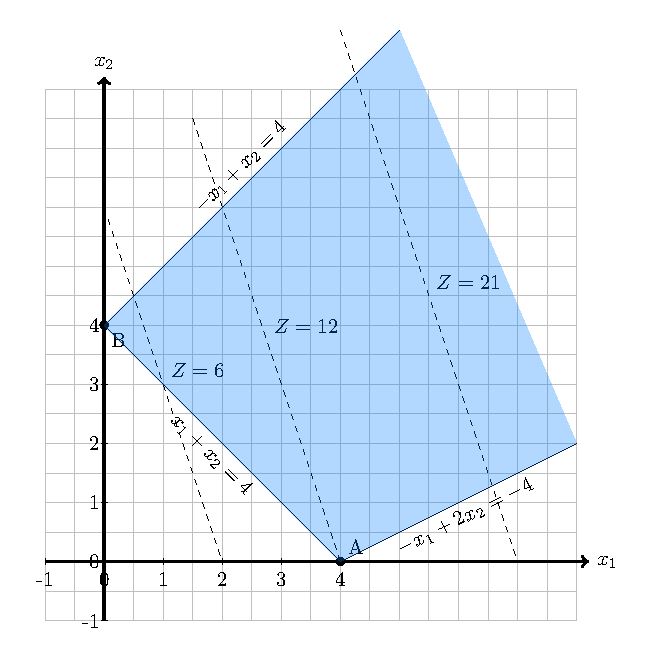
\includegraphics[width=0.7\linewidth]{LP4.pdf}
  \end{center}


  \begin{Exercise}
    \begin{equation*}
      \begin{aligned}
        \text{maximize } \quad & z = 3x_1 + x_2 \\
        \text{subject to }\quad &
        \begin{array}{rcl}
          -x_1 + x_2 &\geq& 4\\
          -x_1 +2x_2 &\leq& -4\\
          x_1,x_2 &\geq &0
        \end{array}
      \end{aligned}
    \end{equation*}
  \end{Exercise}
  \begin{center}
    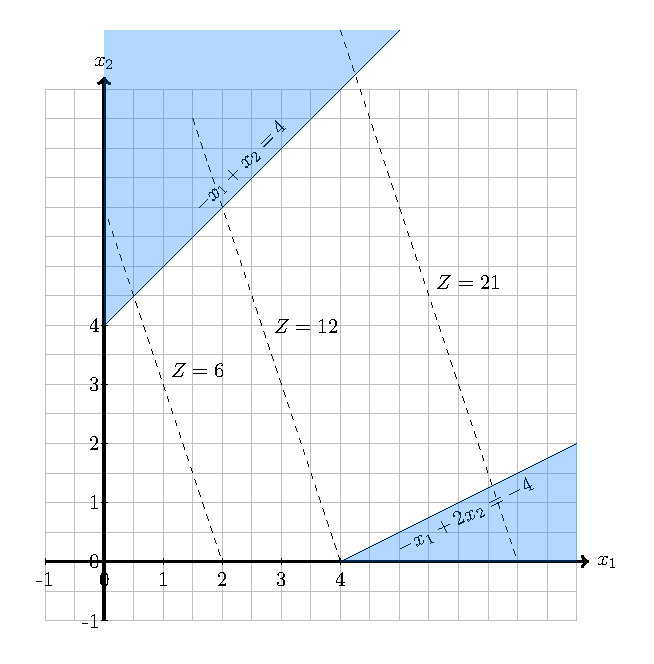
\includegraphics[width=0.7\linewidth]{LP5.pdf}
  \end{center}


\begin{program}
  E4. Build a Python code using Google OR tools' MPSolver interface to solve an arbitrary LP problem. Test it with the different exercises in this presentation.
\end{program}

\subsection{General solution method}

  \begin{itemize}
    \item If an optimal solution exists, it occurs at an extreme point of the feasible region.
    \item Only the finitely many extreme points need be examined (rather than all the points in the feasible region).
    \item Thus, an optimal solution may be found systematically by considering the objective function values at the extreme points.
    \item In fact, in actual practice, only a small subset of the extreme points need be examined.
  \end{itemize}
  This is the foundation for a {\bf general solution method} of a LP problem called the {\bf Simplex method}.

%----------------------------------------------------------------------------------------
